\subsubsection*{Inertial Motion Capture}
\begin{figure}[h]
	\centering
	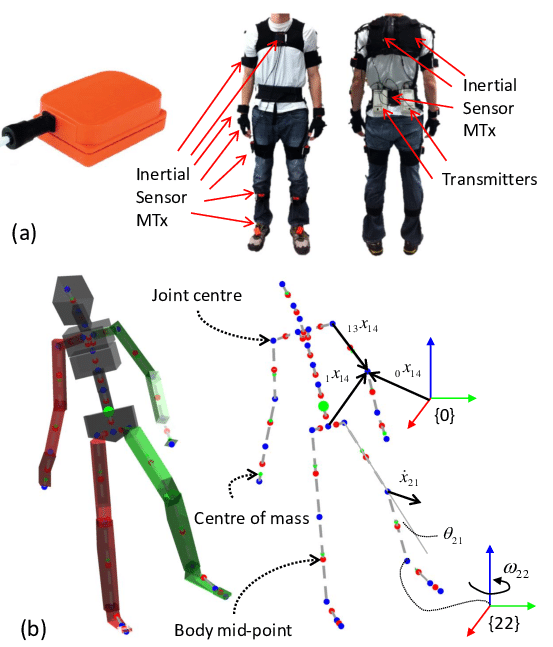
\includegraphics[width=0.4\textwidth]{figures/background/Inertial.png}
	\caption{\href{https://www.researchgate.net/profile/Matthew-Field-6/publication/257308000/figure/fig1/AS:613448983531582@1523269043700/a-The-inertial-sensor-MTx-left-14-and-positioning-of-the-sensors-and-wireless.png}
	{Inertial sensor suit}}
\end{figure}

Inertial sensors \cite{Kalman Filtering for Sensor Fusionin a Human Tracking System} rely on the property of bodies to maintain constant translational and rotational velocity unless perturbed by forces or torques. The vestibular system is a biological 3D inertial sensor located in the inner ear. It can detect both angular motion and linear acceleration of the head. The vestibular system is critical for maintaining eye balance and stabilization in relation to the environment. Advances in miniaturized and micro-machined sensor technologies, particularly silicon accelerometers and rate sensors, have made practical inertial tracking possible. A rate gyroscope measures angular velocity and provides the change in angle with respect to an initially known angle when integrated over time. Accelerations, including gravitational acceleration g, are measured by an accelerometer.\\

If the sensor's angle with respect to the vertical is known, the gravity component can be removed and velocity and position can be calculated using numerical integration. If no compensation is used, the noise and bias errors associated with small and inexpensive sensors make tracking orientation and position for long periods of time impractical. Drift and other errors can be reduced by combining signals from inertial sensors with those from aiding/complementary sensors and using knowledge about their signal characteristics.

\pagebreak

\subsubsection*{Mechanical Motion Capture}

\begin{figure}[h]
	\centering
	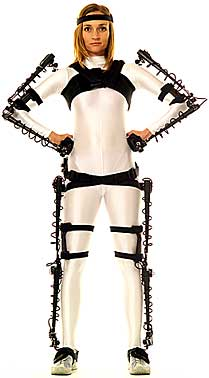
\includegraphics[width=0.3\textwidth]{figures/background/Mechanical.png}
		\caption{\href{https://metamotion.com/images/gypsy4_standing.jpg}
	{Mechanical mocap suit}}
\end{figure}

Because of the external structure \cite{MOTION CAPTURE TO BUILD A FOUNDATION FOR A COMPUTER-CONTROLLED INSTRUMENT BY STUDY OF CLASSICAL GUITAR PERFORMANCE} that is attached to the performer, mechanical motion capture systems are also known as exoskeleton motion capture systems. These structures, which are typically made of rigid metal or plastic, have articulated joints with potentiometers that directly measure a performer's joint angles as he or she moves. One of the primary benefits of this direct measurement system is the absence of the need for cameras or other sensors. The system's main drawbacks are that the performer is restricted to the degrees of freedom of the structure and that the location of the sensor placement is fixed. If the performer attempts to move beyond the system's degrees of freedom, the structure may be damaged or broken.

\pagebreak

\subsubsection*{Magnetic Motion Capture}

\begin{figure}[h]
	\centering
	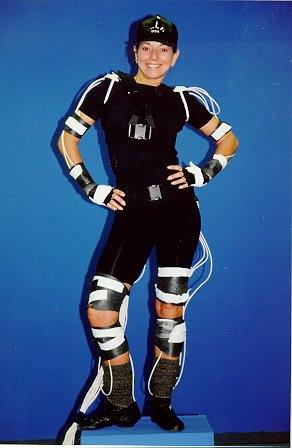
\includegraphics[width=0.3\textwidth]{figures/background/Magnetic.png}
		\caption{\href{https://www.researchgate.net/profile/Jessica-Hodgins-2/publication/2359279/figure/fig4/AS:669524957331457@1536638597171/A-performer-wearing-a-motion-capture-apparatus-The-device-shown-is-a-full-body-magnetic.ppm}
	{Magnetic mocap suit}}
\end{figure}

Magnetic motion capture systems \cite{MOTION CAPTURE TO BUILD A FOUNDATION FOR A COMPUTER-CONTROLLED INSTRUMENT BY STUDY OF CLASSICAL GUITAR PERFORMANCE} work by measuring the low-frequency magnetic field produced by a source transmitter and relaying it to a receiver. Each transmitter and receiver have three orthogonal coils that measure magnetic flux between them and calculate the position and orientation of each sensor. One of the key advantages of these systems is that instead of the more conventional three degrees of position, each sensor transmitter/receiver pair may capture both orientation and position. However, sensors in the system, are susceptible to environmental metal, magnetic fields, and electrical sources such as rebar walls and floors, lights, cables, monitors, and computers. Shielding equipment and wiring requires special care. Despite their high accuracy, the sensors become nonlinear at the extremes of their range.